\chapter{METHODOLOGY}
This chapter will explain the framework, game designs used, content, and evaluation form that we will be using to create and measure the success of this project. The chapter will be divided into 4 parts: System design, Game design, Content, and Evaluation method.

\section{System Design}
Our objective is to create an effective learning application for learning C programming language, so we came to the conclusion that the application should be cross-platformed and easy to use. The framework, React Native, will allow us to cross-platform our application. The framework uses C++ as their main language, so we will using that language for development. Images of the UI will be placed in this section.
    \begin{figure}[!htbp]
    	\centering
    	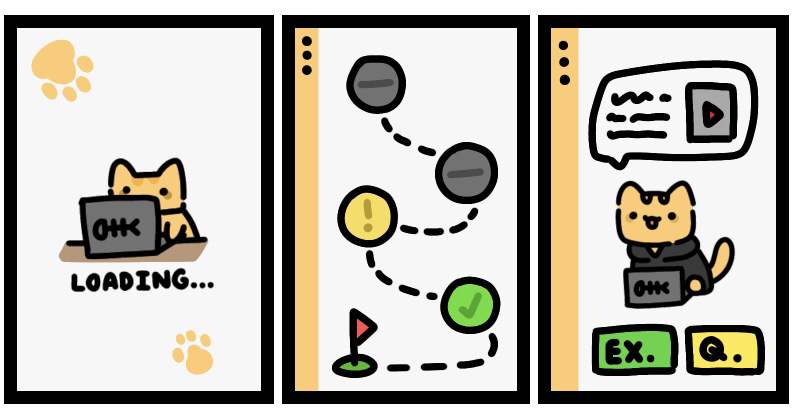
\includegraphics[width = 0.5\textwidth]{UI.png}
    	\caption{Example of the UI}
    	\label{fig:UIExample}
    \end{figure}

\section{Content}
The content that will be used in the game is taken from the class subject EGCI113 - Fundamental Programming. The content will start from simple topics such as type of variable and scanf/printf to more complex topics such as file manipulation. Further topics and details would need to be discussed with our main advisor.

\section{Game Design}
We have thought out the possible types of exercises that will be integrated into the game such as detect the error, code blocking, and fill in the blank (both via typing and drag-\&-drop). We have yet to come to a conclusion on how the lesson part will be presented. We have thought about the lesson being a mixed type where the user will be introduced with the lecture, then they will be led into the exercise part to help them understand and hone their programming skill. We have not yet come up with how the lecture will be presented. Possible integration would be interactive lecture where the mistakes in here will not be counted towards the review calculation and the examples used will be easy for users to understand the basic concept.
	\begin{figure}[!htbp]
		\centering
		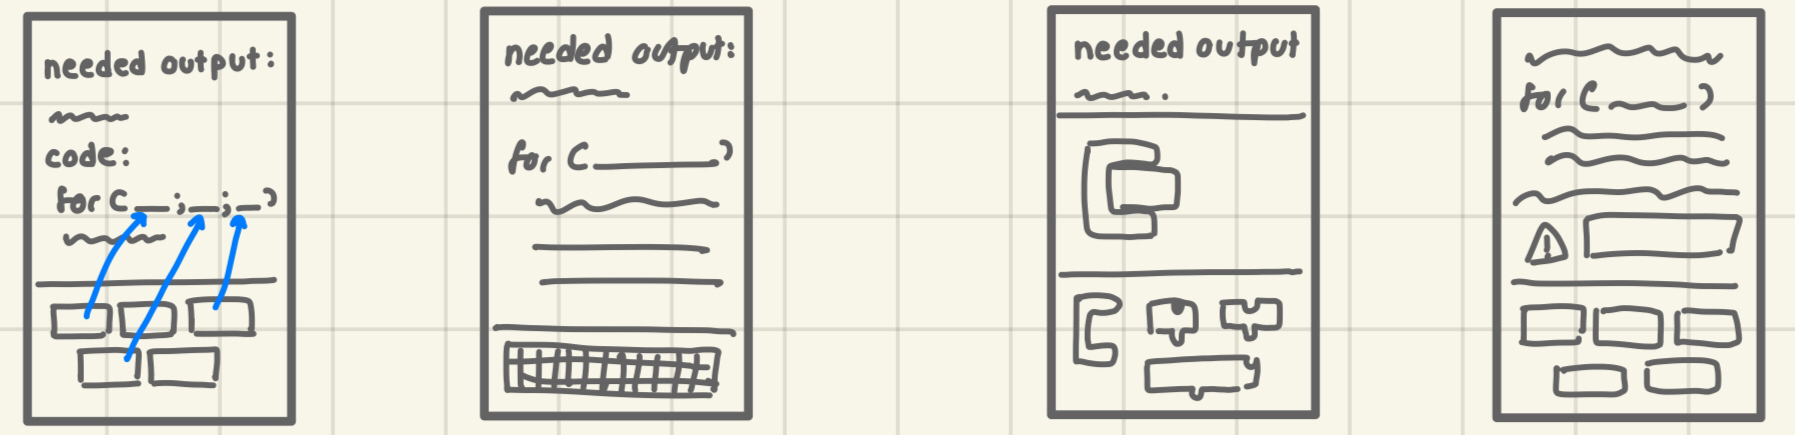
\includegraphics[width = \textwidth]{Exercise.png}
		\caption{Possible Exercises}
		\label{fig:Exercises}
	\end{figure}

\section{Evaluation Method}
Lastly, the evaluation method will possibly be divided into 2 parts: comparison between pure lecture and aided with the application and between our application and other application in the market. We have not yet come up with the sample size or the application that we will be using to compare the result with. Some of the quality that we will use for comparison is engagement. Other possible choices are having pre/post-test and evaluation form.
